\documentclass{article}
\linespread{1.3}
\usepackage[margin=50pt]{geometry}
\usepackage{amsmath, amsthm, amssymb, amsthm, tikz, fancyhdr, graphicx, systeme}
\pagestyle{fancy}
\renewcommand{\headrulewidth}{0pt}
\newcommand{\changefont}{\fontsize{15}{15}\selectfont}

\fancypagestyle{firstpageheader}{
  \fancyhead[R]{
    \changefont
    \parbox[t]{4cm}{ % Adjust width as needed
      Michael Huang\\
      EN.625.603.84\\
      Problem Set \#8
    }
  }
}

\begin{document}

\thispagestyle{firstpageheader}
{\Large 

\section*{11.2.1}
Crickets make their chirping sound by sliding one wing cover very rapidly back and forth over the other. Biologists have long been aware that there is a linear relationship between \(temperature\) and the \(frequency\) with which a cricket chirps, although the slope and y-intercept of the relationship vary from species to species. The following table lists fifteen frequency-temperature observations recorded for the striped ground cricket, \(Nemobius ~ fasciatus ~ fasciatus\) (145). Plot these data and find the equation of the least squares line, \(y = a+bx\). Suppose a cricket of this species is observed to chirp eighteen times per second. What would be the estimated temperature?
\\
\\
We plot the data and line using Python, but can also derive the least squares line with slope \(b\) and intercept \(a\) like so:
\[
b = \frac{n\sum_{i=1}^n x_i y_i - (\sum_{i=1}^n x_i) (\sum_{i=1}^{n} y_i)}{n(\sum_{i=1}^n x_i^2) - (\sum_{i=1}^{n} x_i)^2} = \frac{15 \cdot 20,127.47 - 249.8 \cdot 1,200.6}{15 \cdot 4,200.56 - 249.8^2}
\]
\[
= \frac{301912.05 - 299909.88}{63008.4 - 62400.04} = \frac{2002.17}{608.36} = 3.29109408903
\]
\[
a = \frac{\sum_{i=1}^{n} y_i - b \sum_{i=1}^{n}x_i}{n} = \frac{1,200.6 - 3.29109408903 \cdot 249.8}{15}
\]
\[
= \frac{378.48469656}{15} = 25.232313104
\]
So the least squares line is \(y = a + bx = 25.232313104 + 3.29109408903x\). So we can estimate the temperature to be 
\[
= 25.232313104 + 3.29109408903 \cdot 18 = 84.4719936025
\]
\\
\\
\begin{figure}[h!]
  \centering
  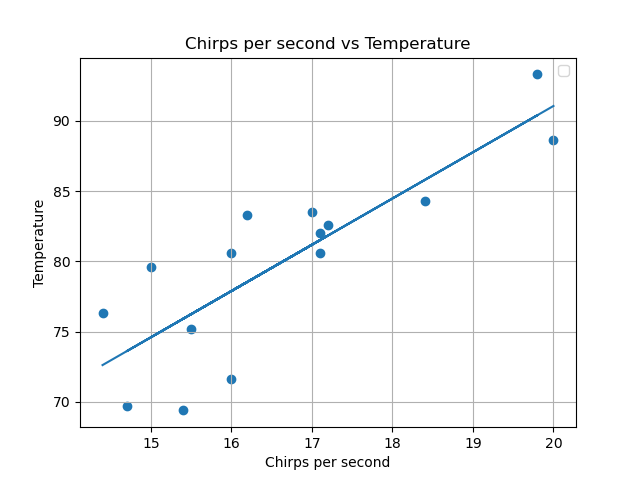
\includegraphics[width=500pt]{cricket_1121.png}
\end{figure}
\\
\\
\\ \\ \\ \\
The code I used is as follows:
\begin{verbatim}
import matplotlib.pyplot as plt
import numpy as np

chirps = np.array([20.0, 16.0, 19.8, 18.4, 17.1, 15.5, 14.7, 17.1, 15.4, 16.2, 15.0, 17.2, 16.0, 17.0, 14.4])
temperatures = np.array([88.6, 71.6, 93.3, 84.3, 80.6, 75.2, 69.7, 82.0, 69.4, 83.3, 79.6, 82.6, 80.6, 83.5, 76.3])

b, a = np.polyfit(chirps, temperatures, deg=1)

y = a + b * chirps 

plt.scatter(chirps, temperatures)
plt.plot(chirps, y)

plt.xlabel("Chirps per second")
plt.ylabel("Temperature")
plt.title("Chirps per second vs Temperature")
plt.legend()
plt.grid(True)
plt.show()\end{verbatim}

\section*{11.2.2}
The aging of whisky in charred oak barrels brings about a number of chemical changes that enhance its taste and darken its color. The following table shows the change in a whisky's proof as a function of the number of years it is stored (168). Graph these
data and draw in the least squares line.
\\
\\
We plot the data and line using Python, but can also derive the least squares line with slope \(b\) and intercept \(a\) like so:
\[
b = \frac{n\sum_{i=1}^n x_i y_i - (\sum_{i=1}^n x_i) (\sum_{i=1}^{n} y_i)}{n(\sum_{i=1}^n x_i^2) - (\sum_{i=1}^{n} x_i)^2} = \frac{10 \cdot 3973.35 - 36.5 \cdot 1070.0}{10 \cdot 204.25 - 36.5^2}
\]
\[
= \frac{39733.5 - 39055}{2042.5 - 1332.25} = \frac{678.5}{710.25} = 0.95529743048
\]
\[
a = \frac{\sum_{i=1}^{n} y_i - b \sum_{i=1}^{n}x_i}{n} = \frac{1070.0 - 0.95529743048 \cdot 36.5}{10}
\]
\[
= \frac{1035.13164379}{10} = 103.513164379
\]
So the least squares line is \(y = a + bx = 103.513164379 + 0.95529743048x\) as displayed in the graph.
\\
\\
\begin{figure}[h!]
  \centering
  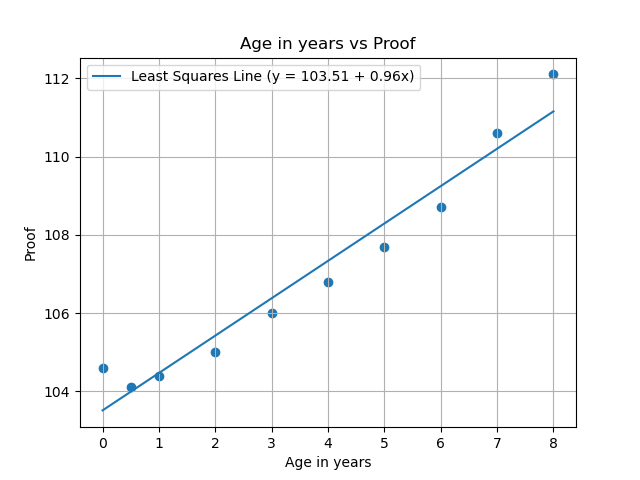
\includegraphics[width=500pt]{whisky_1122.png}
\end{figure}
\\
\\
The code I used is as follows:
\begin{verbatim}
import matplotlib.pyplot as plt
import numpy as np

ages = np.array([0, 0.5, 1, 2, 3, 4, 5, 6, 7, 8])
proofs = np.array([104.6, 104.1, 104.4, 105.0, 106.0, 106.8, 107.7, 108.7, 110.6, 112.1])

n = len(ages)
xy_sum = sum([age * proofs[idx] for idx, age in enumerate(ages)])
x_sum = ages.sum()
y_sum = proofs.sum()
x_squared_sum = sum([age * age for age in ages])

print(f"{n=}")
print(f"{xy_sum=}")
print(f"{x_sum=}")
print(f"{y_sum=}")
print(f"{x_squared_sum=}")

b, a = np.polyfit(ages, proofs, deg=1)

y = a + b * ages 

plt.scatter(ages, proofs)
plt.plot(ages, y, label=f"Least Squares Line (y = {a:.2f} + {b:.2f}x)")

plt.xlabel("Age in years")
plt.ylabel("Proof")
plt.title("Age in years vs Proof")
plt.legend()
plt.grid(True)
plt.show()
\end{verbatim}

\section*{11.2.3}
As water temperature increases, sodium nitrate (NaN\(\text{O}_3\)) becomes more soluble. The following table (110) gives the number of parts of sodium nitrate that dissolve in one hundred parts of water. Calculate the residuals, \(y_1 - \hat{y}_1, \dots, y_9 - \hat{y}_9\), and draw the residual plot. Does it suggest that fitting a straight line through these data would be appropriate?
\\
\\
We can find the corresponding equation for the least squares line and residuals using Python, but we can also derive slope \(b\) and intercept \(a\) like so:
\[
b = \frac{n\sum_{i=1}^n x_i y_i - (\sum_{i=1}^n x_i) (\sum_{i=1}^{n} y_i)}{n(\sum_{i=1}^n x_i^2) - (\sum_{i=1}^{n} x_i)^2} = \frac{9 \cdot 24628.6 - 234 \cdot 811.3}{9 \cdot 10144 - 234^2}
\]
\[
= \frac{221657.4 - 189844.2}{91296 - 54756} = \frac{31813.2}{36540} = 0.87064039408
\]
\[
a = \frac{\sum_{i=1}^{n} y_i - b \sum_{i=1}^{n}x_i}{n} = \frac{811.3 - 0.87064039408 \cdot 234}{9}
\]
\[
= \frac{607.570147785}{9} = 67.5077941983
\]
So the least squares line is \(y = a + bx = 67.5077941983 + 0.8706403940x\). We can then find the residuals by plugging in each temperature value in as \(x\), and then subtracting the actual value from each, which yields the points as plotted below. We see from the graph that the residuals don't really stay around 0, so the straight line may be the greatest for the data. This is because to have the straight line fit well we'd want the residuals or differences between the modeled data on the line and actual data to be pretty close to 0 across the board. 
\\
\\
\begin{figure}[h!]
  \centering
  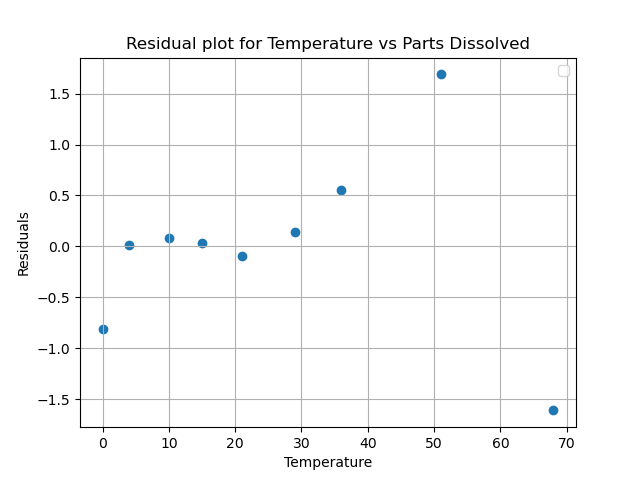
\includegraphics[width=500pt]{water_1123.png}
\end{figure}
\\
\\
\\ \\ \\ \\ \\ \\ \\ \\ \\ \\ \\ \\ \\
The code I used is as follows:
\begin{verbatim}
import matplotlib.pyplot as plt
import numpy as np

temperatures = np.array([0, 4, 10, 15, 21, 29, 36, 51, 68])
parts = np.array([66.7, 71.0, 76.3, 80.6, 85.7, 92.9, 99.4, 113.6, 125.1])

b, a = np.polyfit(temperatures, parts, deg=1)

y = a + b * temperatures 

residuals = parts - y

plt.scatter(temperatures, residuals)
plt.xlabel("Temperature")
plt.ylabel("Residuals")
plt.title("Residual plot for Temperature vs Parts Dissolved")
plt.legend()
plt.grid(True)
plt.show()
\end{verbatim}

\section*{11.2.7}
The relationship between school funding and student performance continues to be a hotly debated political and philosophical issue. Typical of the data available are the following figures, showing the per-pupil expenditures and graduation rate for twenty-six randomly chosen districts in Massachusetts. Graph the data and superimpose the least squares line, \(y = a + bx\).
\\
\\
We plot the data and line using Python, but we can also derive the least squares line with slope \(b\) and intercept \(a\) like so:
\[
b = \frac{n\sum_{i=1}^n x_i y_i - (\sum_{i=1}^n x_i) (\sum_{i=1}^{n} y_i)}{n(\sum_{i=1}^n x_i^2) - (\sum_{i=1}^{n} x_i)^2} = \frac{26 \cdot 31,402  - 360 \cdot 2,256.6}{26 \cdot 5,365.08 - 360^2}
\]
\[
= \frac{816452 - 812376}{139492.08 - 129600} = \frac{4076}{9892.08} = 0.41204680916
\]
\[
a = \frac{\sum_{i=1}^{n} y_i - b \sum_{i=1}^{n}x_i}{n} = \frac{2,256.6 - 0.41204680916 \cdot 360}{26}
\]
\[
= \frac{2108.2631487}{26} = 81.0870441808
\]
So the least squares line is \(y = a + bx = 103.513164379 + 0.41204680916x\) as displayed in the graph.
\\
\\
\begin{figure}[h!]
  \centering
  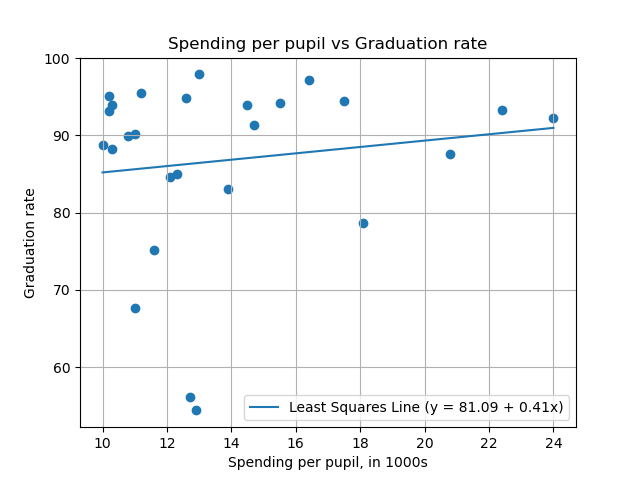
\includegraphics[width=500pt]{school_1127.png}
\end{figure}
\\
\\
The code I used is as follows:
\begin{verbatim}
import matplotlib.pyplot as plt
import numpy as np

spendings = np.array([10.0, 10.2, 10.2, 10.3, 10.3, 10.8, 11.0, 11.0, 11.2, 11.6, 12.1, 12.3, 12.6, 12.7, 12.9, 13.0, 13.9, 14.5, 14.7, 15.5, 16.4, 17.5, 18.1, 20.8, 22.4, 24.0 ])
rates = np.array([88.7, 93.2, 95.1, 94.0, 88.3, 89.9, 67.7, 90.2, 95.5, 75.2, 84.6, 85.0, 94.8, 56.1, 54.4, 97.9, 83.0, 94.0, 91.4, 94.2, 97.2, 94.4, 78.6, 87.6, 93.3, 92.3])

b, a = np.polyfit(spendings, rates, deg=1)

y = a + b * spendings 

plt.scatter(spendings, rates)
plt.plot(spendings, y, label=f"Least Squares Line (y = {a:.2f} + {b:.2f}x)")

plt.xlabel("Spending per pupil, in 1000s")
plt.ylabel("Graduation rate")
plt.title("Spending per pupil vs Graduation rate")
plt.legend()
plt.grid(True)
plt.show()
\end{verbatim}

\section*{11.2.13}
Prove that a least squares straight line must necessarily
pass through the point \(( \bar{x}, \bar{y})\).
\\
\\
By definition, we know that 
\[
a = \frac{\sum_{i=1}^{n} y_i - b \sum_{i=1}^{n}x_i}{n} = \bar{y} - b \bar{x}
\]
We can just subtitute in for the least squares straight line quation \(y = a + bx\) and find that 
\[
y = a + b\bar{x}
\]
\[
y = \bar{y} - b\bar{x} + b x
\]
\[
y - \bar{y} = b(x - \bar{x})
\]
Taking the value for \(x = \bar{x}\):
\[
y - \bar{y} = b(\bar{x} - \bar{x})
\]
\[
y - \bar{y} = 0
\]
\[
y = \bar{y}
\]
So the corresponding \(y\)-value for \(x = \bar{x}\) is \(\bar{y}\), so when graphed the line must pass therefore pass through the point \((\bar{x}, \bar{y})\).

\section*{11.2.14}
In some regression situations, there are \(a ~ priori\) reasons for assuming that the \(xy\)-relationship being approximated passes through the origin. If so, the equation to be fit to the \((x_i, y_i)\)'s has the form \(y = bx\). Use the least squares criterion to show that the “best” slope in that case is given by 
\[
b = \frac{\sum_{i=1}^n x_i y_i}{\sum_{i=1}^{n} x_i^2}
\]
\\
\\
By definition, the least squares criterion means that we find the best slope by minimizing for 
\[
L = \sum_{i=1}^{n} [y_i - (a + bx_i)]^2
\]
Since we are going through the origin, then we have intercept \(a = 0\), so we are minimizing 
\[
L = \sum_{i=1}^{n} (y_i - bx_i)^2
\]
We can find the minimum by differentiating for b and setting the derivative to 0:
\[
\frac{dL}{db} = 0 = \sum_{i=1}^{n} 2 \cdot (y_i - bx_i) \cdot -x_i
\]
\[
0 = -2 \sum_{i=1}^{n} x_i(y_i - bx_i)
\]
\[
0 = \sum_{i=1}^{n} x_i y_i - \sum_{i=1}^{n} bx_i^2
\]
\[
b\sum_{i=1}^{n} x_i^2 = \sum_{i=1}^{n} x_i y_i
\]
\[
b = \frac{\sum_{i=1}^{n} x_i y_i }{\sum_{i=1}^{n} x_i^2}
\]
exactly as we had hoped to find.

\section*{11.3.2}
The best straight line through the Massachusetts funding/graduation rate data described in Question 11.2.7 has the equation y = 81.088+0.412x, where s = 11.78848.

\subsection*{(a)} 
Construct a 95\% confidence interval for \(\beta_1\).
\\
\\
We know by definition that the interval for the confidence interval can be evaluated as 
\[
\big[ \hat{\beta_1} - t_{\alpha / 2, n - 2} \cdot \frac{s}{\sqrt{\sum_{i=1}^{n}(x_i - \bar{x})^2}}, \hat{\beta_1} + t_{\alpha / 2, n - 2} \cdot \frac{s}{\sqrt{\sum_{i=1}^{n}(x_i - \bar{x})^2}} \big]
\]
We are given summary statistics related to \(x_i\), \(\hat{\beta_1} = 0.412\), and \(\alpha = 1 - 0.95 = 0.05\), and we can also intuitively find that \(\bar{x} = \frac{360}{26} = 13.8461538462\) and 
\[
\sum_{i=1}^{n}(x_i - \bar{x})^2 = \sum_{i=1}^{n}x_i^2 - \frac{(\sum_{i=1}^{n} x_i)^2}{n}
\]
\[
= 5365.08 - \frac{360^2}{26} = 5365.08 - 4984.61538462 = 380.46461538
\]
We can thus substitute to find the confidence interval to be
\[
\big[ 0.412 - t_{0.05 / 2, 26 - 2} \cdot \frac{11.78848}{\sqrt{380.46461538}}, 0.412 + t_{0.05 / 2, 26 - 2} \cdot \frac{11.78848}{\sqrt{380.46461538}} \big]
\]
\[
\big[ 0.412 - t_{0.025, 24} \cdot \frac{11.78848}{19.5055021822}, 0.412 + t_{0.025, 24} \cdot \frac{11.78848}{19.5055021822} \big]
\]
\[
\big[ 0.412 - 2.064 \cdot 0.6043669058, 0.412 + 2.064 \cdot 0.6043669058 \big]
\]
\[
\big[-0.83541329357, 1.65941329357\big]
\]

\subsection*{(b)}
What does your answer to part (a) imply about the outcome of testing \(H_0: \beta_1 = 0\) versus \(H_1: \beta_1 \neq 0\) at the \(\alpha = 0.05\) level of significance?
\\
\\
We find that the confidence interval for \(\beta_1\) includes 0, which means that we don't have statistically significant evidence at \(\alpha = 0.05\) to reject \(H_0\), i.e. there is not enough evidence to say that \(\beta_1\) is not equal to 0.

\section*{11.3.14}
Construct a 90\% confidence interval for \(\sigma^2\) in the cigarette-consumption/CHD mortality data given in Case Study 11.3.1.
\\
\\
We know from the conclusion of the case study that the observations satisfy the properties of a simple linear model. We therefore know \(P[\frac{(n-2)S^2}{\chi^2_{1-\alpha / 2, n-2}} \leq \sigma^2 \leq \frac{(n-2)S^2}{\chi^2_{\alpha / 2, n-2}}] = 1 - \alpha\). We are given that \(n=21\) and the corresponding calculations of the relevant sum values for \(x_i\) and \(y_i\) from the table. Let's use this to calculate the confidence interval with \(\alpha = 1 - 0.9 = 0.1\): 
\[
\big(\frac{(n-2)S^2}{\chi^2_{1-\alpha / 2, n-2}}, \frac{(n-2)S^2}{\chi^2_{\alpha / 2, n-2}}\big)
\]
\[
\big(\frac{(n-2)(\frac{1}{n-1}(\sum_{i=1}^{n}y_i^2 - \frac{(\sum_{i=1}^{n}y_i)^2}{n}))}{\chi^2_{1-\alpha / 2, n-2}}, \frac{(n-2)(\frac{1}{n-1}(\sum_{i=1}^{n}y_i^2 - \frac{(\sum_{i=1}^{n}y_i)}{n}))}{\chi^2_{\alpha / 2, n-2}}\big)
\]
\[
\big(\frac{(21-2)(\frac{1}{21-1} (529,321.58 - \frac{3042.2^2}{21}))}{\chi^2_{1 - 0.05, 21-2}}, \frac{(21-2)(\frac{1}{21-1} (529,321.58 - \frac{3042.2^2}{21}))}{\chi^2_{0.05, 21-2}}\big)
\]
\[
\big(\frac{19 \cdot (\frac{1}{20} \cdot 88608.206667)}{\chi^2_{0.95, 19}}, \frac{19 \cdot (\frac{1}{20} \cdot 88608.206667)}{\chi^2_{0.05, 19}}\big)
\]
Looking up the values in a chi squared table:
\[
\big(\frac{84177.7963336}{31.410}, \frac{84177.7963336}{10.117}\big)
\]
\[
\big(2679.96804628, 8320.43059539 \big)
\]
which is therefore our 90\% confidence interval for the population variance of the data.

\section*{11.3.16}
Regression techniques can be very useful in situationswhere one variable—say, \(y\)—is difficult to measure but \(x\) is not. Once such an \(xy\)-relationship has been “calibrated," based on a set of \((x_i, y_i)\)'s, future values of \(Y\) can be easily estimated using \(\hat{\beta}_0 + \hat{\beta}_1x\). Determining the volume of an irregularly shaped object, for example, is often difficult, but weighing that object is likely to be easy. The following table shows the weights (in kilograms) and the volumes (in cubic decimeters) of eighteen children between the ages of five and eight (15). The estimated regression line has the equation \(y = -0.104+0.988x\), where \(s = 0.202\).

\subsection*{(a)} 
Construct a 95\% confidence interval for \(E(Y | 14.0)\).
\\
\\
We calculate some of the 
The middle point \(\hat{y}\) for the confidence interval as found by the equation is 
\[
\hat{y} = -0.104 + 0.988 \cdot 14.0 = 13.832 - 0.104 = 13.728 
\]
and to find the intervals around this value, we know by definition that 
\[
w = t_{\alpha / 2, n - 2} \cdot s \sqrt{\frac{1}{n} + \frac{(x - \bar{x})^2}{\sum_{i=1}^{n}(x_i - \bar{x})^2}}
\]
\[
= t_{0.05 / 2, 18 - 2} \cdot 0.202 \cdot \sqrt{\frac{1}{18} + \frac{(14.0 - 15.005555555555556)^2}{96.38944444444444}}
\]
\[
= t_{0.025, 16} \cdot 0.202 \cdot \sqrt{\frac{1}{18} + \frac{1.01114197532}{96.38944444444444}}
\]
\[
= 2.120 \cdot 0.202 \cdot \sqrt{0.06604572883}
\]
\[
= 0.11005495458
\]
So the confidence interval would be
\[
(13.728 - 0.11005495458, 13.728 + 0.11005495458)
\]
\[
(13.6179450454, 13.8380549546)
\]

\subsection*{(b)} 
Construct a 95\% prediction interval for the volume of a child weighing 14.0 kilograms.
\\
\\
Similar to part (a), we find \(\hat{y}, \bar{x} \), and \(\sum_{i=1}^{n} (x_i - \bar{x})^2\). We then use definition for predicting for \(Y = 14.0\) to find the interval values around \(\hat{y}\) to be 
\[
w = t_{\alpha / 2, n - 2} \cdot s \cdot \sqrt{1 + \frac{1}{n} + \frac{(x - \bar{x})^2}{\sum_{i=1}^{n}(x_i - \bar{x})^2}}
\]
\[
= t_{0.05 / 2, 18 - 2} \cdot 0.202 \cdot \sqrt{1 + \frac{1}{18} + \frac{(14.0 - 15.005555555555556)^2}{96.38944444444444}}
\]
\[
= t_{0.025, 16} \cdot 0.202 \cdot \sqrt{1 + \frac{1}{18} + \frac{1.01114197532}{96.38944444444444}}
\]
\[
= 2.120 \cdot 0.202 \cdot \sqrt{1.06604572883}
\]
\[
= 0.44215561811
\]
So the confidence interval would be 
\[
(13.728 - 0.44215561811, 13.728 + 0.44215561811)
\]
\[
(13.2858443819, 14.1701556181)
\]
\\
\\
The code I used for these two parts is as follows:
\begin{verbatim}
import numpy as np

weights = [17.1, 10.5, 13.8, 15.7, 11.9, 10.4, 15.0, 16.0, 17.8, 15.8, 15.1, 12.1, 18.4, 17.1, 16.7, 16.5, 15.1, 15.1]
volumes = [16.7, 10.4, 13.5, 15.7, 11.6, 10.2, 14.5, 15.8, 17.6, 15.2, 14.8, 11.9, 18.3, 16.7, 16.6, 15.9, 15.1, 14.5]

mean_weight = np.mean(weights)
weight_squares_sum = np.sum([np.square(weight - mean_weight) for weight in weights])

print(f"{mean_weight=}")
print(f"{weight_squares_sum=}")
\end{verbatim}
with the following output:
\begin{verbatim}
~/Doc/e/j/S/Problem Sets/EN.625.603.84/Problem Set 8 problem-set-8 *1 .......................................... py base 15:02:09
> python volume_11316.py 
mean_weight=np.float64(15.005555555555556)
weight_squares_sum=np.float64(96.38944444444444)
\end{verbatim}

\section*{11.3.17}
Construct a 95\% confidence interval for \(E(Y | 2.750) \) using the connecting rod data given in Case Study 11.2.1.
\\
\\
We know from the table that \(n = 25, \sum_{i=1}^{25} x_i = 66.075, \sum_{i=1}^{25} x_i^2 = 174.692925\), which easily lends to finding \(\bar{x} = 66.075 \div 25 = 2.643\) and 
\[
\sum_{i=1}^{25} (x_i - \bar{x})^2 = \sum_{i=1}^{25} x_i^2 - \bar{x}^2 - 2x_i\bar{x}
\]
\[
= \sum_{i=1}^{25} x_i^2 - \sum_{i=1}^{25} \bar{x}^2 - 2\sum_{i=1}^{25} x_i \bar{x}
\]
\[
= \sum_{i=1}^{25} x_i^2 - \sum_{i=1}^{25} \bar{x}^2 - 2\bar{x}\sum_{i=1}^{25} x_i 
\]
\[
= 174.692925 + 25 \cdot 2.643^2 - 2 \cdot 2.643 \cdot 66.075
\]
\[
= 174.692925 + 174.636225 - 349.27245
\]
\[
= 0.0567
\]
We can now by definition use the least squarees line found in the case study to find that 
\[
\hat{y} = 0.308 + 0.642x 
\]
\[
\hat{y} = 0.308 + 0.642 \cdot 2.750
\]
\[
\hat{y} = 2.0735
\]
and that 
\[
w = t_{\alpha / 2, n - 2} \cdot s \sqrt{\frac{1}{n} + \frac{(x - \bar{x})^2}{\sum_{i=1}^{n}(x_i - \bar{x})^2}}
\]
\[
= t_{0.05 / 2, 25 - 2} \cdot \sqrt{\frac{\sum_{i=1}^{25}(x_i - \bar{x}^2)}{n-1}} \cdot \sqrt{\frac{1}{25} + \frac{(2.750  - 2.643)^2}{0.0567}}
\]
\[
= t_{0.025, 23} \cdot \sqrt{\frac{0.0567}{25-1}} \cdot \sqrt{\frac{1}{25} + \frac{0.011449}{0.0567}}
\]
\[
= 2.069 \cdot \sqrt{0.0023625} \cdot \sqrt{0.24192239858}
\]
\[
= 0.04946345393
\]
So the confidence interval is 
\[
(2.0735 - 0.04946345393, 2.0735 + 0.04946345393)
\]
\[
(2.02403654607, 2.12296345393)
\]

\section*{11.4.12}
Many people believe that a salary bonus is a reward for good performance. The corporate world may have a different understanding. A random sample of thirty chief executive officers of large capitalization public companies recorded the cash bonus paid, \(x\) (in \$100,000), and the performance of the company, \(y\), as measured by percentage change in company revenues. The following sums resulted. Find the sample coefficient of correlation. What does this study say about the relationship between bonuses and performance?
\\
\\
Given the values, we know that We know by definition that the sample correlation coefficient is 
\[
R = \frac{n \sum_{i=1}^{n} X_i Y_i - (\sum_{i=1}^{n} X_i)(\sum_{i=1}^{n}Y_i)}{\sqrt{n \sum_{i=1}^{n} X_i^2 - (\sum_{i=1}^{n} X_i)^2} \sqrt{n\sum_{i=1}^{n}Y_i^2 - (\sum_{i=1}^{n} Y_i)^2}}
\]
\[
= \frac{30 \cdot 7807.36 - 1300.69 \cdot 323}{\sqrt{30 \cdot 86754.6939 - 1300.69^2}\sqrt{30 \cdot 11881 - 323^2}}
\]
\[
= \frac{234220.8 - 420122.87}{\sqrt{2602640.817 - 1691794.4761}\sqrt{356430 - 104329}}
\]
\[
\frac{-185902.07}{954.382701488 \cdot 502.096604251} = -0.38794877283
\]
so this implies a slightly weak negative correlation, which means that there is a slight trend of CEOs of companies with poorer performance getting higher bonuses.

\section*{11.4.15}
A common saying in golf is “You drive for show,but you putt for dough.” To see if there is any truth in this assertion, data for ninety-six top money-winning golfers were examined. For each, their money earnings in 2014 (\(y\), in \$ millions), their average yards per drive (\(v\)), and their average number of putts (\(x\)) were tallied.

\subsection*{(a)} 
Show that the correlation coefficient between the
putting average and earnings reveal a slightly stronger relationship than that for driving and earnings.
\\
\\


\subsection*{(b)} 
For each correlation \(r\), compute \(r^2\) to show that neither the \(v\) nor the \(x\) variable alone is a good predictor of earnings.
\\
\\


% End of the large subsection
}

\end{document}